\input{preamble.tex}
\usepackage{makecell} % commande \thead, dans l'exo 1
\usepackage{eurosym} % pour le symbole euro propre

\begin{document}

\reversemarginpar

\pagestyle{fancy}
\fancyhead[L]{Terminale STMG}
\fancyhead[C]{\textbf{Préparation DS n°5.2 (chapitre 4)}}
\fancyhead[R]{\today}

\null\vspace{-30pt}
Nom / Prénom : \\

Consignes particulières : 
\begin{itemize}[label=$\bullet$]
	\item 
	La calculatrice est {autorisée}.
	\item 
	L'exercice \ref{exe:1} peut être fait entièrement sur la feuille.
	\item 
	Ce devoir \textbf{n'est pas noté} il a vocation à vous préparer.
\end{itemize}

\hrule

\exe{5}{
Esquisser la représentation graphique de la fonction inverse dans le repère ci-dessous :
\begin{center}
	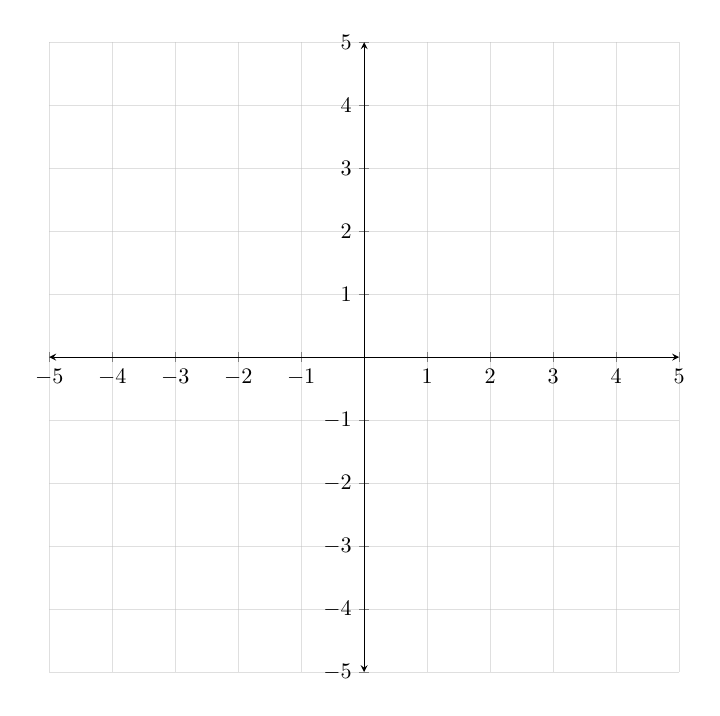
\begin{tikzpicture}[>=stealth, scale=.8]
		\begin{axis}[xmin = -5, xmax=5, ymin=-5, ymax=5, axis x line=middle, axis y line=middle, axis line style=<->, xlabel={}, ylabel={}, grid=both, grid style = {opacity=.5}, clip=false, xtick distance = 1, ytick distance=1, x=1cm, y=1cm]
		\end{axis}
	\end{tikzpicture}
\end{center}
Compléter les phrases suivantes :
\begin{multicols}{2}
\begin{enumerate}
\item $\lim\limits_{x \to - \infty} \dfrac1{x} = \dots$
\item $\lim\limits_{\substack{x \to 0 \\ x <0 }} \dfrac1{x} = \dots$
\item $\lim\limits_{\substack{x \to 0 \\ x >0 }} \dfrac1{x} = \dots$
\item $\lim\limits_{x \to + \infty} \dfrac1{x} = \dots$
\end{enumerate}
\end{multicols}
}{exe:1}{
Voir cours.
}

\exe{5}{
On considère la fonction $f$ définie sur $\R$ par $f(x) = -x^3 + \frac32 x^2 +18x +5$.
\begin{enumerate}
\item Déterminer la fonction dérivée de $f$ sur $\R$.
\item Montrer que l'on peut écrire :
\[ f'(x) = -3(x-3)(x+2) \]
\item En déduire les valeurs $x$ pour lesquels $f'(x)=0$.
\item Dresser le tableau de variation de $f$ sur $\R$.
\end{enumerate}
}{exe:2}{
\begin{enumerate}
\item $f'(x) = -3x^2+3x+18$
\item Il suffit de développer l'expression donnée.
\item $x=3$ et $x=-2$.
\item 
\begin{center}
\begin{tikzpicture}
   \tkzTabInit{$x$ / 1 , $f'(x)$ / 1, $f(x)$ / 1.5}{$-\infty$, $-2$, $3$, $\infty$}
   \tkzTabLine{, -, z, +, z, -, }
   \tkzTabVar{ +/ $+\infty$, -/ , +/, -/ $-\infty$ }
\end{tikzpicture}
\end{center}
\end{enumerate}
}

\exe{5}{
On considère la fonction $g$ définie sur $\Ret$ par $g(x) = 2x - 3 + \frac{72}{x}$.
\begin{enumerate}
\item Déterminer la fonction dérivée de $g$ sur $\Ret$.
\item Montrer que l'on peut écrire :
\[ g'(x) = \dfrac{2(x-6)(x+6)}{x^2} \]
\item En déduire les valeurs $x$ pour lesquels $g'(x)=0$.
\item Etudier les limites éventuelles de $g$ sur son ensemble de définition.
\item Dresser le tableau de variation de $g$ sur $\Ret$.
\end{enumerate}
}{exe:3}{
\begin{enumerate}
\item $g'(x)=2-\frac{72}{x^2}$
\item Il suffit de développer.
\item $x=-6$ ou $x=6$
\item On trouve :
\begin{align*}
\lim_{x \to - \infty} g(x) & = - \infty & \lim_{x \to + \infty} g(x) & = + \infty \\
\lim_{\substack{x \to 0 \\ x <0 }} g(x) & = - \infty & \lim_{\substack{x \to 0 \\ x >0 }} g(x) & = + \infty
\end{align*}
\item
\begin{center}
\begin{tikzpicture}
   \tkzTabInit{$x$ / 1 , $f'(x)$ / 1, $f(x)$ / 1.5}{$-\infty$, $-9$, $0$, $9$, $+\infty$}
   \tkzTabLine{, +, z, -, d, -, z, +, }
   \tkzTabVar{-/ $-\infty$ , +/, -D+/ $-\infty$ / $+\infty$, -/, +/ $+\infty$ }
\end{tikzpicture}
\end{center}
\end{enumerate}
}

\exe{5}{
Une entreprise fabrique chaque jour entre 5 $m^3$ et 60 $m^3$ d'engrais liquide.
Le coût moyen quotidien de production (exprimé en centaines d'euros) de cet engrais est modélisé par la fonction :
\[ \begin{array}{c c c c}
f : & \R & \to & \R \\
& x & \mapsto & x - 15 + \dfrac{400}{x} \end{array} \]
où la variable $x$ correspond au volume d'engrais produit (en $m^3$).
\begin{enumerate}
\item En considérant la production de l'usine, donner les valeurs possibles pour la variable $x$ ? 
Exprimer la réponse sous forme d'un intervalle.
\item Déterminer la dérivée de la fonction $f$.
\item Montrer que l'on peut écrire :
\[ f'(x) = \dfrac{(x-20)(x+20)}{x^2} . \]
\item Dresser le tableau de variation de $f$. Restreindre ce tableau aux valeurs de $x$ cohérentes avec la production de l'entreprise.
\item Pour quel volume d'engrais produit le coût moyen quotidien de prodution est-il minimal ? Quel est ce coût moyen minimal ?
\end{enumerate}
}{exe:4}{
\begin{enumerate}
\item $x \in [5 ;60]$.
\item $f'(x) = 1 - \dfrac{400}{x^2}$.
\item $\dfrac{(x-20)(x+20)}{x^2} = \dfrac{x^2 - 400}{x^2} = f'(x)$.
\item 
\begin{center}
\begin{tikzpicture}
   \tkzTabInit{$x$ / 1 , $f'(x)$ / 1, $f(x)$ / 1.5}{$5$, $20$, $60$}
   \tkzTabLine{, -, z, +,}
   \tkzTabVar{+/ , -/, +/ }
\end{tikzpicture}
\end{center}
\item La fonction atteint un minimum sur [5 ;60] en $x=20$ (donc 20 $m^3$ d'engrais) et $f(20)=25$, 
soit un coût moyen minimal de 2~500 \euro.
\end{enumerate}
}

%%%%%%%%%%%%

\newpage
\fancyhead[C]{\textbf{Solutions}}
\shipoutAnswer


\end{document}
